% !TeX program = xelatex
% !BIB program = bibtex
\makeatletter
\def\input@path{{template/}}
\makeatother

\documentclass{sbc2019}
\usepackage{booktabs}
\usepackage{graphicx}
\usepackage[table]{xcolor}
\usepackage{tikz}
\usepackage{fontawesome}
\usepackage{academicons}
\usepackage{hyperref}
\usepackage[bottom]{footmisc}
\usetikzlibrary{arrows.meta,positioning,shapes.geometric,calc,fit}

\definecolor{darkblue}{rgb}{0.0,0.0,0.0}
\hypersetup{
  colorlinks,
  breaklinks,
  linkcolor=darkblue,
  urlcolor=darkblue,
  anchorcolor=darkblue,
  citecolor=darkblue
}

% Journal metadata for the submission version. Volume, issue, year, and DOI
% are intentionally omitted because they are assigned during publication.
\jid{JSERD}
\jtitle{Journal of Software Engineering Research and Development}
\copyrightstatement{This work is licensed under a Creative Commons Attribution 4.0 International License}

\begin{document}

\title[HalluCodeDetection]{HalluCodeDetection: Detecting Hallucinations in Code Generation}

% TODO before submission: include the author's ORCID, institutional affiliation
% (using its official English name), and contact email in this affiliation block.
\author[de Lima]{
  \affil{\textbf{Rubens Nascimento de Lima}}
}

\begin{frontmatter}
\maketitle

\begin{abstract}
\textbf{Abstract}

Abstract goes here.
\end{abstract}

\begin{keywords}
Code Generation, Hallucination Detection, Small Language Models, Static Analysis
\end{keywords}
\end{frontmatter}

\section{Introduction}
\label{sec:introduction}

Large language models have become increasingly capable of generating executable source code from natural-language specifications, making code generation one of the most prominent applications of generative AI in software engineering. However, plausible-looking code is not necessarily correct. Generated programs may violate the syntax of the programming language, fail during execution, or execute normally while deviating from the intended functionality. These failures are increasingly discussed as \emph{code hallucinations}: outputs that appear plausible but are incorrect or inconsistent with the requested behavior~\citep{pavel2025hallucination,lee2025hallucination}. \citet{lee2025hallucination}, for example, distinguish syntactic, runtime-execution, functional-correctness, and code-quality hallucinations. In this study, we focus on the first three categories, which correspond to observable failures in correctness and executability. Understanding and detecting these failures is important because generated code can appear convincing enough to be accepted by a developer even when its behavior is incorrect, transferring part of the verification burden from code generation to code assessment.

Detecting such hallucinations is itself a difficult problem. Syntax errors can often be identified mechanically, but executable code may fail only for particular inputs or silently return incorrect results. Empirical studies have shown that functional failures represent an important fraction of errors produced by code-generation models, while different models exhibit substantially different failure distributions~\citep{dou2025whatswrong,tian2025codehalu}. Test execution can provide an objective oracle when sufficiently strong test cases are available, but a model evaluating generated code does not necessarily have access to those tests or to execution results. Moreover, generating correct code and recognizing incorrect code are distinct capabilities: a model that performs well as a generator may still be a poor evaluator of its own or another model's output. This motivates studying hallucination detection as a task in its own right rather than treating correctness assessment only as a by-product of code generation.

We investigate this problem from the perspective of \emph{Small Language Models} (SLMs). Our central idea is to evaluate whether compact models can not only generate code, but also act as hallucination detectors, and whether task specialization can compensate for limited model scale. Rather than reducing verification to a binary correct/incorrect decision, we formulate hallucination detection as a multilabel classification task over \emph{Syntax}, \emph{Runtime}, \emph{Functional}, and \emph{Correct}. A generated solution may contain both runtime and functional failures when different test cases expose different behaviors, while \emph{Correct} is reserved for solutions that successfully satisfy the complete evaluation suite. This formulation allows us to study not only whether an SLM recognizes that a program is wrong, but also which forms of hallucination it is capable of identifying. We further examine whether models can recognize errors in code that they generated themselves and whether a specialized SLM can provide a more reliable detector than general-purpose models.

Our study follows a controlled experimental pipeline built on the 563 programming tasks of EvalPlus~\citep{liu2023evalplus}. Multiple SLMs first generate one solution for each task, and the resulting programs are compiled and executed against the strengthened HumanEval and MBPP test suites to construct an execution-based multilabel ground truth. The same task descriptions and generated programs are then presented to the models without test results or reference labels, turning hallucination detection into an independent evaluation task. To investigate specialization, we construct a supervised dataset through knowledge distillation: three teacher models independently receive the execution-derived labels and produce natural-language rationales explaining the corresponding failures. These rationales are used as auxiliary supervision when fine-tuning Gemma-based models with QLoRA, while the quantitative evaluation remains based solely on the predicted classes. We evaluate different optimization strategies to account for the strong class imbalance in the dataset and compare the resulting specialized detectors with both general-purpose SLMs and substantially larger models under the same detection protocol. Finally, we investigate whether conventional static-analysis signals from Python compilation and Pyright can complement model-based generation and hallucination detection.

The results reveal a clear separation between code-generation capability and hallucination-detection capability. Across the evaluated SLMs, code-generation correctness ranges from 62\% to 81\%, with functional hallucinations being considerably more frequent than syntax failures. Error detection is substantially more heterogeneous: the best general-purpose SLM reaches 73.1\% exact-set Accuracy and 53.8\% Macro-F1, while no general-purpose model detects more than approximately one third of the Runtime errors. Models also differ substantially in their ability to recognize their own failures; self-error detection ranges from only 5.3\% for GPT-OSS 20B to 69.3\% for Qwen 3.8 27B, showing that strong generation does not imply strong self-evaluation. Specialized training substantially improves detection: the Accuracy-oriented model reaches 77.8\% Accuracy, a gain of 31.9 percentage points over its base model, while Macro-F1-oriented training reaches 54.2\% Macro-F1 and provides a more balanced error profile. Moreover, the specialized SLMs remain competitive with models that are an order of magnitude larger: the best specialized detector surpasses both evaluated large models in Macro-F1, while the Accuracy-oriented detector also achieves the highest Accuracy. These results indicate that task specialization can partially compensate for model scale, although Runtime hallucinations remain challenging across all evaluated model groups.

% TODO RQ5: After the tool-assisted experiments are finalized, add one or two sentences here summarizing the strongest result regarding (i) static analysis alone, (ii) tool-assisted code generation, and/or (iii) tool-assisted hallucination detection. Prefer a concrete improvement/regression value rather than a qualitative statement.

The main contributions of this work are:
\begin{itemize}
    \item An empirical evaluation of the code-generation and hallucination-detection capabilities of SLMs under a common execution-based ground truth, distinguishing syntactic, runtime, and functional failures through multilabel classification.
    \item An analysis of \emph{self-error detection}, measuring whether models can recognize the hallucinations present in code that they generated themselves and showing that generation and self-evaluation capabilities do not necessarily coincide.
    \item A specialized SLM-based hallucination detector trained with execution-derived labels and teacher-generated rationales, together with an analysis of how different optimization objectives and class-imbalance strategies affect its detection behavior.
    \item A controlled comparison between general-purpose SLMs, specialized SLMs, and substantially larger language models under the same detection protocol, showing that increased scale does not guarantee superior hallucination detection.
    \item An investigation of the complementarity between model-based reasoning and traditional static-analysis evidence, considering static tools both as feedback during code generation and as supporting evidence during hallucination detection.
\end{itemize}

The remainder of this paper is organized as follows. Section~\ref{sec:related-work} reviews existing work on code hallucinations, empirical failure characterization, automatic code evaluation, specialized critics, and feedback-guided code generation. Section~\ref{sec:methodology} describes the evaluated models, generation protocol, execution-based ground truth, hallucination-detection task, knowledge-distillation procedure, specialized training, evaluation metrics, and integration with static-analysis tools. The subsequent sections present the empirical results for code generation, general hallucination detection and self-evaluation, specialized detection, comparison with larger models, and tool-assisted approaches. Finally, the paper discusses the implications and limitations of the findings and summarizes the main conclusions.

\section{Related Work}
\label{sec:related-work}

\subsection{Hallucinations in code generation}

The term \emph{hallucination} has no single, universally accepted operational definition in code generation.  \citet{pavel2025hallucination} characterize it as an output that appears plausible but is factually incorrect, unverifiable, or nonsensical, and document syntax violations, invalid references, and API-knowledge conflicts in an automotive case study.  This definition is useful because plausibility alone is not evidence that generated code compiles, runs, or fulfills its specification.

\citet{lee2025hallucination} survey code-generation hallucinations and organize them into syntactic, runtime-execution, functional-correctness, and code-quality hallucinations.  We adopt the first three observable-error classes: a syntactic hallucination violates the language grammar; a runtime hallucination prevents normal execution; and a functional-correctness hallucination executes but does not satisfy the task specification.  Code quality is deliberately outside the scope of HalluCodeDetection, whose target is correctness and executability rather than style, maintainability, or efficiency.

Other taxonomies make clear that these labels should be treated as an evaluation-oriented abstraction rather than as a claim that all defects have one cause.  CodeHalu defines code hallucinations through execution-based verification and groups them as mapping, naming, resource, and logical hallucinations~\citep{tian2025codehalu}.  These categories emphasize the origin or manifestation of an error, whereas our labels describe the directly observable outcome of generated code.  The two perspectives are therefore complementary: a naming hallucination, for example, may surface as either a runtime failure or a functional failure depending on how it is used.

\subsection{Empirical evidence on failures in generated code}

Empirical studies show that errors in generated code extend beyond simple compilation failures.  \citet{dou2025whatswrong} evaluate closed- and open-source LLMs across three benchmarks, report that harder problems remain challenging, and derive a taxonomy with three bug categories and ten subcategories.  Their real-world benchmark also shows that error distributions can differ from those observed on standard benchmarks.  This motivates reporting error types explicitly instead of relying only on aggregate pass rates.

The automotive study of \citet{pavel2025hallucination} further demonstrates that failures can be tied to domain knowledge and API constraints, even when a prompt is enriched with context.  Together, these studies motivate evaluating whether a detector generalizes across error modes and model families, rather than assuming that one benchmark or one generator captures the whole failure distribution.

\subsection{Automatic evaluation and error detection}

Execution against tests remains a direct oracle for syntax, runtime, and many functional failures.  EvalPlus augments code-generation benchmarks with automatically generated tests and shows that the original tests can miss incorrect programs and even mis-rank models~\citep{liu2023evalplus}.  Accordingly, the labels used by HalluCodeDetection should be grounded in compilation and execution results together with strengthened tests wherever possible; a passing small test suite must not be interpreted as proof of semantic correctness.

CodeHalu operationalizes this idea with dynamic, execution-based verification and introduces CodeHaluEval, a benchmark containing 8,883 samples from 699 tasks~\citep{tian2025codehalu}.  It is closely related because it detects and quantifies code hallucinations, but it uses a heuristic procedure and a taxonomy different from the three outcome classes used here.  HalluCodeDetection instead frames detection as supervised multi-label classification of observable syntactic, runtime, and functional errors.

The closest detector-oriented comparison is \citet{andriushchenko-etal-2026-efficient}, who construct line-level hallucination annotations and train a lightweight Transformer detector using LLM internal representations.  Their work establishes that specialized detectors can outperform generic uncertainty baselines and may support subsequent self-correction.  HalluCodeDetection is complementary in target granularity: it predicts error categories for generated code, rather than locating hallucinated lines, and evaluates the role of specialized small language models and tool-derived evidence.

\subsection{Specialized critics and rationale-based feedback}

Learned evaluators have also been used as components of the generation loop.  CodeRL trains a critic to predict functional correctness and uses unit-test feedback and critic scores to guide regeneration~\citep{le2022coderl}.  Its outcome space includes compile errors, runtime errors, failed tests, and passed tests, which makes it a particularly relevant precedent for distinguishing observable failure modes.  However, CodeRL optimizes a generator through reinforcement learning; it is not a stand-alone, multi-label hallucination detector.

This distinction matters for the positioning of HalluCodeDetection.  The contribution is not the broad idea of using a model to assess code---learned critics and detector models already exist---but the proposed supervised detector specialized for the selected hallucination taxonomy, its rationale-oriented training, and its empirical comparison with larger general-purpose models and tool-assisted signals.

\subsection{Self-evaluation, self-correction, and tool-assisted generation}

Several lines of work use feedback to revise an initial output.  Self-Refine iterates generation, self-feedback, and refinement without additional training~\citep{madaan2023selfrefine}, while Reflexion stores verbal reflections on feedback for later trials and includes coding tasks~\citep{shinn2023reflexion}.  These frameworks establish the general value of iterative feedback, but their feedback need not be a reliable, explicitly typed code-error diagnosis.

For code specifically, Self-Debugging prompts an LLM to inspect execution results and explain its program before revising it~\citep{chen2024selfdebug}.  \citet{dou2025whatswrong} likewise propose a training-free loop using self-critique, bug types, and compiler feedback.  These approaches are complementary to HalluCodeDetection: tools such as compilers, interpreters, and tests can provide high-precision evidence when they are applicable, while a specialized detector can provide a typed warning when a full oracle is unavailable, incomplete, or too expensive to run.

Thus, the article should avoid claiming that generation--evaluation--correction loops are new.  Its defensible distinction is the evaluated combination of a supervised, multi-label hallucination detector for syntactic, runtime, and functional failures; a focus on small specialized models; and tool-assisted evidence used alongside, rather than substituted for, detector predictions.

\section{Methodology}
\label{sec:methodology}

\subsection{Study Overview}
\label{sec:study_overview}

This study investigates the ability of Small Language Models (SLMs) to both generate correct code and identify errors in code generated by other models. The experiment combines code generation, automated classification, knowledge distillation, and specialized training to evaluate different dimensions of the problem.

Several language models generate solutions for standardized programming tasks. Each solution is executed against a test suite that objectively determines whether the code is correct or contains syntax, runtime, or functional errors. This ground truth classification is used both to evaluate the code generation capability of the models and as the basis for detection experiments.

The study includes a knowledge distillation process in which language models act as judges to generate natural language explanations for each identified error type. These explanations are associated with the reference labels and compose the data used for supervised training of a specialized error detection model via \textit{fine-tuning} with the QLoRA technique.

Detection capability is evaluated for both general-purpose models, without specific training, and the specialized model. In both cases, the model receives only the programming task description and the generated code, without access to reference labels or test execution results.

The detection task is treated as multilabel classification, since the same code may contain more than one type of error simultaneously.

\subsection{Evaluated Models}
\label{sec:evaluated_models}

The study evaluates language models with parameter counts ranging from 4B to 552B, as shown in Table~\ref{tab:models}. The table separates the small language models that are the main focus of the study from the two large models used only for the comparison with larger models.

\begin{table}[htbp]
\centering
\caption{Models evaluated in the study}
\label{tab:models}
\begin{tabular}{lc}
\toprule
\textbf{Model} & \textbf{Parameters} \\
\midrule
\multicolumn{2}{l}{\textit{Small language models}} \\
\midrule
Devstral Small 2 & \shortstack[c]{24B\\{\scriptsize\citep{rastogi2025devstral}}\\{\scriptsize\citep{mistralai2025devstral2}}} \\
GLM 4.7 Flash & \shortstack[c]{30B\\{\scriptsize\citep{glm45team2025glm45}}\\{\scriptsize\citep{zai2025glm47flash}}} \\
Gemma 3 4B & \shortstack[c]{4B\\{\scriptsize\citep{gemmateam2025gemma3}}} \\
Gemma 4 & \shortstack[c]{\{5.1, 8, 31\}B\\{\scriptsize\citep{gemmateam2026gemma4}}} \\
GPT-OSS 20B & \shortstack[c]{20B\\{\scriptsize\citep{openai2025gptoss}}} \\
Muse Glimmer 30B & \shortstack[c]{30B\\{\scriptsize\citep{meta2026museglimmer}}} \\
Ornith 1.5 35B & \shortstack[c]{35B\\{\scriptsize\citep{ornithteam2026ornith15}}} \\
Qwen 2.5 Coder & \shortstack[c]{\{7, 32\}B\\{\scriptsize\citep{hui2024qwen25coder}}} \\
Qwen 3 Coder 30B & \shortstack[c]{30B\\{\scriptsize\citep{yang2025qwen3}}\\{\scriptsize\citep{qwenteam2025qwen3coder}}} \\
Qwen 3.8 27B & \shortstack[c]{27B\\{\scriptsize\citep{qwenteam2026qwen38}}} \\
\midrule
\multicolumn{2}{l}{\textit{Large models (comparison)}} \\
\midrule
DeepSeek V4.1 Flash & \shortstack[c]{552B\\{\scriptsize\citep{deepseekai2026deepseekv41flash}}} \\
MiMo V2.5 & \shortstack[c]{310B\\{\scriptsize\citep{xiaomimimo2026mimov25}}} \\
\bottomrule
\end{tabular}
\end{table}

The local SLMs used in the initial code generation were executed with Q4\_K\_M quantization, which allowed larger models to be evaluated within the available computational budget. The Gemma models were also evaluated without precision reduction in the detection experiments. The fine-tuned models were executed without inference quantization; their adaptation used QLoRA with 4-bit NF4 quantization~\citep{dettmers2023qlora}, which is a training mechanism distinct from Q4\_K\_M inference quantization. The two large models were accessed through a hosted API, so no quantization level is assumed for them.

For the knowledge distillation process, three models were selected as judges: Muse Glimmer 30B, Qwen 3.8 27B, and Ornith 1.5 35B. These models were chosen because they are the largest general-purpose models and demonstrated strong performance in the code generation step.

For the specialized model training, the Gemma 4 E2B and E4B models were used as base models for \textit{fine-tuning}, along with Gemma 3 4B.

During the knowledge distillation and error detection evaluation, all models were configured with a temperature of 0.0 to ensure deterministic outputs. Across all experiments, both the SLMs and the larger comparison models were executed in direct-response mode, with thinking or reasoning mode and reasoning effort disabled whenever these controls were exposed by the model backend. Consequently, the models were not prompted to produce a chain-of-thought or a separate reasoning trace, and no such trace was retained or supplied as input to any subsequent phase.

\subsection{Programming Tasks and Code Generation}
\label{sec:programming_tasks}

The experiments utilize the EvalPlus benchmark~\citep{liu2023evalplus}, which extends both HumanEval~\citep{chen2021humaneval} and MBPP~\citep{austin2021mbpp} with additional test cases to increase the reliability of correctness assessment. EvalPlus provides 164 tasks from HumanEval and 399 tasks from MBPP, totaling 563 programming tasks.

Each task consists of a natural language problem description that specifies the required functionality. The problems cover diverse algorithmic challenges, including string manipulation, mathematical operations, and data structure operations. For HumanEval tasks, the model receives the function signature and must complete the function body. For MBPP tasks, the model generates the complete function implementation.

The code generation process uses a system prompt that instructs the model to act as a Python assistant that solves coding problems, returning only a single function implementation without tests, asserts, or example usage. The user prompt varies according to the benchmark: for HumanEval, it requests the completion of a function body; for MBPP, it requests the complete function implementation.

For the initial code generation, each model produced one solution per programming task, using a temperature of 1.0 to allow for diversity. The top-p and top-k parameters were kept at the defaults of each model or backend, and no fixed random seed was imposed.

The raw response is normalized before execution. The extraction step removes Markdown code fences when they wrap the whole response and detects whether the model already returned the entry-point function definition. For HumanEval completion tasks, the harness reuses the task prompt, which already contains the function header, and appends the normalized function body; when the model returned the complete function definition, that definition is used directly. For MBPP, the returned function definition is used when present; otherwise the required signature is prepended and the body is indented. This normalization does not remove arbitrary natural-language text that the model may produce before or after the code, so a response that mixes prose with code can still fail to compile. When extraction produces an incomplete source, for example when the function header is lost, the ground-truth compilation classifies the solution as Syntax.

\subsection{Ground Truth and Error Classification}
\label{sec:ground_truth}

The ground truth classification is determined by executing each generated solution against a custom test harness that evaluates the code at different levels of correctness. Labels are accumulated across the test cases, so a single solution may receive more than one label, with the exception of Correct.

The procedure starts with a compilation step. If the source cannot be compiled, it receives the Syntax label and the evaluation stops, so Syntax is exclusive and no other label is added. It is important to note that syntax errors may arise from different sources: (1) genuine Python syntax errors in the generated code, such as invalid import statements or malformed expressions; (2) formatting issues, such as the model returning natural language explanations or Markdown fences along with the code; or (3) extraction issues, such as the loss of the function header during code processing.

If the source compiles, it is executed in an isolated subprocess against the base test cases and the additional test cases. For each test case, if the execution raises an exception, the Runtime label is added; if the execution completes but returns a result different from the expected one, the Functional label is added. Runtime and Functional can therefore co-occur in the same solution, because some test cases may raise exceptions while others return incorrect results. A timeout, or a failure that prevents the execution of the candidate as a whole, is also labeled as Runtime.

The Correct label is assigned only when the source compiles, no test case raises an exception, and all test cases return the expected result. It is therefore exclusive: a solution labeled Correct cannot receive any other label, and a solution that receives any error label cannot receive Correct. The procedure is summarized in Figure~\ref{fig:ground_truth}.

\begin{figure}[htbp]
\centering
\begin{minipage}{0.95\columnwidth}
\begin{verbatim}
Input: generated code, EvalPlus tests
labels = {}
if code does not compile:
    labels += Syntax
    return labels
for each test case:
    execute code
    if exception or timeout:
        labels += Runtime
        continue
    if output != expected result:
        labels += Functional
if labels is empty:
    labels += Correct
return labels
\end{verbatim}
\end{minipage}
\caption{Ground truth labeling procedure. Runtime and Functional accumulate across test cases, whereas Syntax terminates the evaluation and Correct is assigned only when no other label is present.}
\label{fig:ground_truth}
\end{figure}

\subsection{Error Detection Experiment}
\label{sec:error_detection}

The error detection experiment evaluates whether language models can correctly identify errors in generated code without access to reference labels or test execution results. For each sample, the model receives only the programming task description and the generated code.

The models are prompted with a system prompt that defines the classification task. Table~\ref{tab:error_types} describes the four error categories used in this study.

\begin{table}[htbp]
\centering
\caption{Error categories and their definitions}
\label{tab:error_types}
% Keep the definitions table within a single column and let the text wrap.
\begin{tabular}{@{}p{0.24\columnwidth}@{}p{0.76\columnwidth}@{}}
\toprule
\textbf{Error Type} & \textbf{Definition} \\
\midrule
Syntax & When the provided code has a syntax error in the Python language, such as incorrect or incomplete code. \\
\midrule
Runtime & When the code is ``compilable'' but has an error when executed, such as a call to an invalid function, an undefined variable, etc. \\
\midrule
Functional & When the code is executable, but it has some deviation from the correct functioning of what was requested. \\
\midrule
Correct & When the code is well-formed and has no functional errors. \\
\bottomrule
\end{tabular}
\end{table}

The prompt instructs the model to return a JSON object containing a list of detected error types, each with a natural language explanation. The prompt emphasizes that the model should provide general explanations without mentioning specific test cases or input values.

All models evaluated in the code generation step are also evaluated in the error detection experiment. The models are evaluated under the same conditions, with a temperature of 0.0 to ensure deterministic outputs. The two large models used in the comparison with larger models follow exactly the same detection protocol as the SLMs: same set of examples, same task description, same input code, same system prompt, same class definitions, same output format, same metrics, and the same temperature. No additional information, tests, or ground truth is provided to them.

The Exact-set Accuracy measures the proportion of samples where the set of predicted error types exactly matches the set of ground truth error types. Additionally, Macro F1 and Macro Recall are computed by isolating each error class independently, providing a per-class analysis of detection capability.

\subsection{Specialized Model Training and Knowledge Distillation}
\label{sec:specialized_training}

This section describes both the knowledge distillation process used to generate training data and the specialized model training procedure.

\subsubsection{Knowledge Distillation}

The knowledge distillation process generates natural language explanations for each error type identified in the ground truth classification. For each generated code sample, a judge model receives the problem description, the generated code, the name of the model that generated the code, and the ground truth error labels. The judge is instructed to write a general explanation for each error type present, describing why the code can fail in that way without mentioning specific test cases or input values. The judge does not assign or correct the label; it explains a label that was already determined by execution.

Every example is processed by all three judges: Muse Glimmer 30B, Qwen 3.8 27B, and Ornith 1.5 35B. These models were chosen because they are the largest general-purpose models and demonstrated strong performance in the code generation step. Each judge produces its own rationale for the same code and the same reference label, and no voting or winner selection is performed. Each generated sample therefore contributes one training record per judge, that is, three records that share the code and the label but carry a different rationale. Each rationale associates an error type with the explanation produced by the judge. If a judge fails to produce a response for a sample, no record is written for that judge and the sample is retried in a later execution. The reference label always comes from the execution of the code, and the rationale is only the target text that accompanies it.

Training the specialized model on the label together with an explanation, rather than on the label alone, provides richer auxiliary supervision. Label-only supervision indicates which output is expected but offers little explicit information about the relation between the task requirement, the behavior of the code, and the error category, which in an imbalanced dataset can favor superficial correlations and shortcuts associated with the dominant class. Conditioning the target on an explanation encourages the model to associate its prediction with evidence in the code. This follows the rationale-based distillation of \citet{hsieh-etal-2023-distilling}, which uses rationales as additional supervision, and the explanation-based fine-tuning of \citet{ludan-etal-2023-explanation}, which reports reduced reliance on spurious cues. The explanations provide richer auxiliary supervision and are not claimed to eliminate bias or to guarantee robustness. In the quantitative evaluation, only the predicted classes enter the metrics; the textual quality of the explanations is not scored.

\subsubsection{Specialized Model Training}

The training dataset is the output of the knowledge distillation process described above. Each record in this dataset contains the problem description, the generated code, and the corresponding error labels with explanations generated by the judge models.

The base models selected for \textit{fine-tuning} are Gemma 4 E2B, Gemma 4 E4B, and Gemma 3 4B. Each training sample is formatted as a three-turn conversation. The system prompt describes the classification task and defines the four error categories. The user message contains the programming task description and the generated code. The assistant message contains the expected output: a JSON object with the detected error types and their explanations, formatted as a Markdown code block.

The training uses QLoRA (Quantized Low-Rank Adaptation) with 4-bit NF4 quantization~\citep{dettmers2023qlora}, applying low-rank adapters as introduced by LoRA~\citep{hu2022lora}. Table~\ref{tab:training_params} shows the hyperparameters explored during the search.

\begin{table}[htbp]
\centering
\caption{Training hyperparameters}
\label{tab:training_params}
\begin{tabular}{ll}
\toprule
\textbf{Parameter} & \textbf{Values} \\
\midrule
LoRA rank ($r$) & \{8, 16, 32\} \\
LoRA alpha ($\alpha$) & \{8, 16, 32\} \\
LoRA dropout & \{0.05, 0.1\} \\
Learning rate & \{5e-5, 1e-4\} \\
Bias & \{none, all, lora\_only\} \\
Epochs & \{3, 4\} \\
\bottomrule
\end{tabular}
\end{table}

The dataset is split into training, validation, and test sets. The split is performed at the task level, so all code samples for a given programming task are assigned to the same split, preventing data leakage where different solutions for the same task appear across splits. The validation set comprises 15\% of the data, and the test set comprises 20\%.

Four training configurations were evaluated. The first two use the original class distribution, without removing Syntax and without explicit balancing. The first is Accuracy-oriented: it uses the standard causal language-modeling loss and selects the best model by validation Accuracy. The second is Macro-F1-oriented: it uses the label-weighted loss, which assigns a higher weight to the class-name tokens, and selects the best model by validation Macro-F1.

The other two configurations balance the training split only. Correct examples are reduced, Syntax examples are removed from training, and the remaining examples are downsampled to a runtime:functional:correct ratio of 1:1:1 or 1:3:3, without duplicating rows. Validation and test remain unchanged, so balancing cannot move a task between splits. Both balanced configurations use the label-weighted loss; the third selects the best model by validation Accuracy, and the fourth by validation Macro-F1.

Hyperparameter search was performed with Optuna~\citep{akiba2019optuna} using the Tree-structured Parzen Estimator (TPE) sampler with multivariate sampling and constant-liar. The search space covers the base model, LoRA rank and alpha, LoRA dropout, learning rate, number of epochs, and bias configuration, as listed in Table~\ref{tab:training_params}. For each search, the best configuration is the one that maximizes the respective selection metric on the validation split, and the corresponding merged adapter is retained.

\subsection{Evaluation Metrics}
\label{sec:evaluation_metrics}

The evaluation uses metrics appropriate for multilabel classification scenarios. For each of the four error categories (syntax, runtime, functional, and correct), true positives (TP), false positives (FP), and false negatives (FN) are computed independently.

The per-class recall is calculated as $TP / (TP + FN)$, measuring the proportion of actual positive cases correctly identified for each error type. The per-class precision is calculated as $TP / (TP + FP)$, measuring the proportion of predicted positive cases that are actually correct.

The Macro F1 score is computed as the average of the F1 scores across all four error categories, where each category's F1 score is $2 \times TP / (2 \times TP + FP + FN)$. This metric treats all error types equally, regardless of their frequency in the dataset.

The Macro Recall is computed as the average of the recall scores across all four error categories, providing a measure of the overall detection capability across error types.

The Exact-set Accuracy measures the proportion of samples where the set of predicted error types exactly matches the set of ground truth error types. This strict metric requires a complete match of the multilabel prediction, reflecting the practical requirement that a detection system must correctly identify all present error types.

\subsection{Static Analysis Tools}
\label{sec:static_tools}

Two static analysis tools are used in this study, each exclusive to one failure category. Python compilation (\texttt{py\_compile}) is responsible for the syntax category, and Pyright is responsible for statically detectable runtime issues.

Python compilation, implemented with the language's built-in \texttt{compile} function~\citep{pythoncompile}, parses the source code into a code object and reports a syntax error when the source cannot be parsed. A compilation failure is mapped to Syntax, whereas a successful compilation is interpreted as the absence of a syntax signal. It is never used to detect Runtime or Functional errors, and it does not execute the code. Because it only parses the source, it is fast and deterministic.

Pyright is a standards-based static type checker for Python~\citep{microsoftpyright} that analyzes the source code without executing it. It builds a model of the program and reports conditions that would fail at execution. In this study it is invoked under the default type checking mode with \texttt{pyright --outputjson --level error --pythonversion 3.13}, so only diagnostics with error severity are parsed. A diagnostic is mapped to Runtime only when its rule belongs to the runtime-related set considered here, which includes \texttt{reportUndefinedVariable}, \texttt{reportUnboundVariable}, \texttt{reportPossiblyUnboundVariable}, \texttt{reportCallIssue}, \texttt{reportArgumentType}, \texttt{reportAssignmentType}, \texttt{reportAttributeAccessIssue}, \texttt{reportIndexIssue}, \texttt{reportOperatorIssue}, \texttt{reportReturnType}, \texttt{reportOptionalCall}, \texttt{reportOptionalMemberAccess}, \texttt{reportOptionalOperand}, \texttt{reportOptionalSubscript}, \texttt{reportOptionalIterable}, \texttt{reportOptionalContextManager}, \texttt{reportOptionalEnter}, \texttt{reportGeneralTypeIssues}, and \texttt{reportInvalidTypeArguments}. Diagnostics without a rule whose message indicates a parsing problem, such as an expected token or an indentation error, are mapped to Syntax. All other diagnostics, including style and type-annotation warnings, are ignored. Pyright detects runtime issues that compilation cannot, but it cannot detect functional errors, since these depend on the expected behavior of the program. If a tool fails to run or produces output that cannot be parsed, the failure is recorded as a tool error and no prediction is derived from it.

\subsection{Interactive Cycles with Tools}
\label{sec:interactive_cycles}

Two experiments use the static tools in their loop: one for code generation and one for code verification. Figures~\ref{fig:cycle_generation} and~\ref{fig:cycle_verification} summarize both flows.

\subsubsection{For Code Generation}

\begin{figure}[htbp]
\centering
\resizebox{0.6\columnwidth}{!}{%
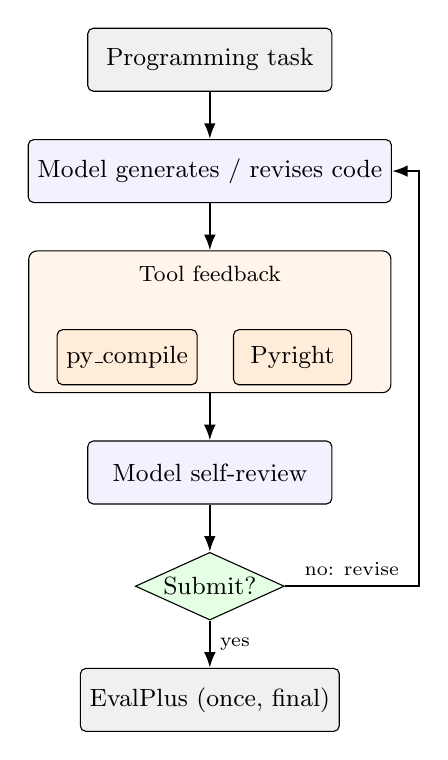
\begin{tikzpicture}[
  font=\small,
  box/.style={draw, rounded corners=2pt, align=center, minimum width=3.1cm, minimum height=0.8cm, fill=blue!5},
  subtool/.style={draw, rounded corners=2pt, align=center, minimum width=1.5cm, minimum height=0.7cm, fill=orange!15},
  container/.style={draw, rounded corners=3pt, fill=orange!8, minimum width=4.6cm, minimum height=1.8cm},
  dec/.style={draw, diamond, aspect=2.2, align=center, inner sep=1pt, fill=green!10},
  term/.style={draw, rounded corners=2pt, align=center, minimum width=3.1cm, minimum height=0.8cm, fill=gray!12},
  arr/.style={-{Latex[length=2mm]}, thick},
  lbl/.style={font=\scriptsize}
]
\node[term] (g0) at (0,0) {Programming task};
\node[box]  (g1) [below=6mm of g0] {Model generates / revises code};
\node[container] (tf) [below=6mm of g1] {};
\node[font=\footnotesize] at ([yshift=-3mm]tf.north) {Tool feedback};
\node[subtool] at ([xshift=-1.05cm,yshift=-4.5mm]tf.center) {py\_compile};
\node[subtool] at ([xshift=1.05cm,yshift=-4.5mm]tf.center) {Pyright};
\node[box]  (g3) [below=6mm of tf] {Model self-review};
\node[dec]  (g4) [below=6mm of g3] {Submit?};
\node[term] (g5) [below=6mm of g4] {EvalPlus (once, final)};
\draw[arr] (g0)--(g1);
\draw[arr] (g1)--(tf);
\draw[arr] (tf)--(g3);
\draw[arr] (g3)--(g4);
\draw[arr] (g4)--node[lbl,right]{yes}(g5);
\draw[arr] (g4.east) -- ++(1.7,0) node[lbl,above,pos=0.5]{no: revise} |- (g1.east);
\end{tikzpicture}%
}
\caption{Code generation cycle. The model iterates between generation, static analysis, and self-review, and EvalPlus is applied only to the final candidate.}
\label{fig:cycle_generation}
\end{figure}

In the generation cycle, the model first produces an initial solution for a programming task. In each round, the candidate is analyzed by Python compilation and, only when it compiles, by Pyright, so the tools run in a short-circuit order and a candidate that does not compile does not reach Pyright. The resulting diagnostics are returned to the model, which performs a self-review and may either submit the current solution or return a revised implementation, following the broader paradigm of iterative self-feedback and self-debugging~\citep{madaan2023selfrefine,chen2024selfdebug}. The prompt contains only the task, the current candidate, and the current feedback; the full history of previous rounds is not provided. When no diagnostic is found, the feedback states that no syntax or statically detectable runtime issue was reported and still asks the model to assess the code, so the model may revise even without diagnostics. When the model revises, the returned implementation completely replaces the candidate, without any correctness validation before the substitution, and the cycle repeats, and when the model does not return the requested JSON, a code-only fallback is used. The cycle stops when the model submits or when the maximum of five rounds is reached, and both the generation and the review use a temperature of 0. The evaluation with EvalPlus is applied only once, to the final candidate, and its result is never included in any generation or self-review prompt, so the model has no access to the test outcome during the cycle. Because a revision is not guaranteed to be better than the previous candidate, the process is also analyzed in terms of improved, unchanged, and regressed outcomes, and regressions are retained rather than discarded.

\subsubsection{For Code Verification}

In the verification experiment, the model receives the programming task description and a held-out solution generated during the initial code generation, together with the static feedback produced by Python compilation and Pyright for that solution. This experiment is a controlled comparison: the same model, on the same sample, is evaluated with and without the static feedback. The version without feedback corresponds to the general error detection experiment, and the two versions share the same task, the same code, the same base prompt, the same temperature, and the same metrics, so only the static feedback differs. The feedback is presented as supporting evidence and never as a ground truth label. It is a short text that reports the compile status and, when the source compiles, the Pyright runtime status, followed by the diagnostics; when no issue is found, it states that no syntax or statically detectable runtime issue was reported and adds that this does not prove functional correctness. The prompt states that the tools can be incomplete, that the absence of a diagnostic does not imply that the code is correct, and that the tools do not detect functional errors in general. The model then returns the multilabel classification of the code into syntax, runtime, functional, and correct. The static feedback is used only as evidence for the classification and never replaces the reference labels, which are used exclusively afterward to compute the metrics.

\begin{figure}[htbp]
\centering
\resizebox{0.6\columnwidth}{!}{%
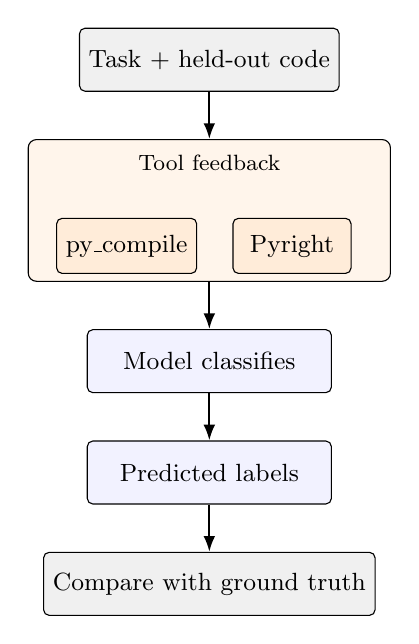
\begin{tikzpicture}[
  font=\small,
  box/.style={draw, rounded corners=2pt, align=center, minimum width=3.1cm, minimum height=0.8cm, fill=blue!5},
  subtool/.style={draw, rounded corners=2pt, align=center, minimum width=1.5cm, minimum height=0.7cm, fill=orange!15},
  container/.style={draw, rounded corners=3pt, fill=orange!8, minimum width=4.6cm, minimum height=1.8cm},
  term/.style={draw, rounded corners=2pt, align=center, minimum width=3.1cm, minimum height=0.8cm, fill=gray!12},
  arr/.style={-{Latex[length=2mm]}, thick}
]
\node[term] (v0) at (0,0) {Task + held-out code};
\node[container] (tf) [below=6mm of v0] {};
\node[font=\footnotesize] at ([yshift=-3mm]tf.north) {Tool feedback};
\node[subtool] at ([xshift=-1.05cm,yshift=-4.5mm]tf.center) {py\_compile};
\node[subtool] at ([xshift=1.05cm,yshift=-4.5mm]tf.center) {Pyright};
\node[box] (v3) [below=6mm of tf] {Model classifies};
\node[box] (v4) [below=6mm of v3] {Predicted labels};
\node[term] (v5) [below=6mm of v4] {Compare with ground truth};
\draw[arr] (v0)--(tf);
\draw[arr] (tf)--(v3);
\draw[arr] (v3)--(v4);
\draw[arr] (v4)--(v5);
\end{tikzpicture}%
}
\caption{Code verification cycle. The model classifies held-out code using the static feedback as supporting evidence.}
\label{fig:cycle_verification}
\end{figure}


\section{Results and Discussion}
\label{sec:results}
\subsection{RQ1: To what extent can different language models generate correct code?}
\label{sec:rq1}

\newcommand{\score}[1]{%
  \ifdim #1pt < 25pt \cellcolor{red!20}#1%
  \else\ifdim #1pt < 50pt \cellcolor{orange!20}#1%
  \else\ifdim #1pt < 75pt \cellcolor{yellow!30}#1%
  \else\cellcolor{green!30}#1%
  \fi\fi\fi%
}

\newcommand{\scorecell}[2]{%
  \ifdim #1pt < 25pt \cellcolor{red!20}#2%
  \else\ifdim #1pt < 50pt \cellcolor{orange!20}#2%
  \else\ifdim #1pt < 75pt \cellcolor{yellow!30}#2%
  \else\cellcolor{green!30}#2%
  \fi\fi\fi%
}

\begin{table}[htbp]
\centering
\caption{Code generation results by model across the 563 programming tasks of EvalPlus}
\label{tab:rq1_generation}
\setlength{\tabcolsep}{3pt}
\newcommand{\lightmodelrule}{%
  \arrayrulecolor{black!15}\specialrule{0.25pt}{0.5pt}{0.5pt}\arrayrulecolor{black}%
}
\begin{tabular}{@{}>{\centering\arraybackslash}m{0.31\columnwidth}*{4}{>{\centering\arraybackslash}m{0.1475\columnwidth}}@{}}
\toprule
\small\textbf{Model} & \small\textbf{Correct} & \small\textbf{Funct.} & \small\textbf{Runtime} & \small\textbf{Syntax} \\
\midrule
\multicolumn{5}{l}{\textit{Small language models}} \\
\midrule
\shortstack[c]{Muse Glimmer\\(30B)} & \textbf{81\%} & \textbf{15\%} & \textbf{4\%} & 1\% \\
\lightmodelrule
\shortstack[c]{GPT-OSS\\(20B)} & 79\% & 17\% & 5\% & 0\% \\
\lightmodelrule
\shortstack[c]{Gemma 4\\(31B)} & 79\% & 15\% & 4\% & 3\% \\
\lightmodelrule
\shortstack[c]{Qwen 3 Coder\\(30B)} & 77\% & 18\% & 6\% & 1\% \\
\lightmodelrule
\shortstack[c]{Qwen 3.8\\(27B)} & 76\% & 19\% & 6\% & 0\% \\
\lightmodelrule
\shortstack[c]{Qwen 2.5 Coder\\(7B)} & 73\% & 21\% & 8\% & 0\% \\
\lightmodelrule
\shortstack[c]{Devstral Small 2\\(24B)} & 71\% & 24\% & 7\% & 0\% \\
\lightmodelrule
\shortstack[c]{Qwen 2.5 Coder\\(32B)} & 67\% & 25\% & 9\% & 1\% \\
\lightmodelrule
\shortstack[c]{GLM 4.7 Flash\\(30B)} & 66\% & 29\% & 7\% & 0\% \\
\lightmodelrule
\shortstack[c]{Ornith 1.5\\(35B)} & 66\% & 19\% & 7\% & 10\% \\
\lightmodelrule
\shortstack[c]{Gemma 3\\(4B)} & 62\% & 33\% & 9\% & 0\% \\
\midrule
\multicolumn{5}{l}{\textit{Large language models}} \\
\midrule
\shortstack[c]{DeepSeek V4.1\\Flash\\(552B)} & 73\% & 17\% & 6\% & 6\% \\
\lightmodelrule
\shortstack[c]{MiMo V2.5\\(310B)} & 73\% & 19\% & 7\% & 2\% \\
\bottomrule
\end{tabular}

\footnotesize{* Due to the multilabel classification, Functional and Runtime may appear more than once per sample, so the sum of columns may exceed 100\%.}
\end{table}

The first question of this study concerns the ability of language models to generate valid code, with the large models included as external comparison baselines. All evaluated models produced correct code for the majority of tasks, with correctness rates ranging from 62\% to 81\%. This represents a difference of 19 percentage points between the best and worst performing models. Muse Glimmer 30B achieved the highest correctness rate (81\%, corresponding to 456 of 563 tasks), while Gemma 3 4B achieved the lowest (62\%, corresponding to 350 tasks). GPT-OSS 20B and Gemma 4 31B also performed strongly, with 79\% correctness (445 and 443 tasks, respectively).

Regarding model size and performance, larger parameter counts did not consistently translate into higher correctness rates among the evaluated models. Although several of the best-performing models have relatively large parameter counts, model size alone does not explain the observed performance differences. A notable example is the Qwen 2.5 Coder family, where the smaller 7B model achieved 73\% correctness (413 tasks), compared with 67\% (378 tasks) for its 32B counterpart. The 7B model correctly solved 82 tasks that the 32B model failed, while the 32B model correctly solved 47 tasks that the 7B model failed. This difference was significant before correction ($p = 0.0026$), but not after applying Holm correction across all 78 pairwise comparisons ($p_{\mathrm{adj}} = 0.091$); it should therefore be interpreted as descriptive evidence rather than a confirmed pairwise difference.

The large-model baselines reinforce this weak relationship between parameter count and code-generation performance. DeepSeek V4.1 Flash and MiMo V2.5 each solved 413 of the 563 tasks (73.4\%), exactly matching the number of correct solutions produced by Qwen 2.5 Coder 7B. Their correctness was also close to Qwen 3.8 27B (76\%) and Devstral Small 2 24B (71\%), while remaining below the best SLMs, Muse Glimmer 30B (81\%), GPT-OSS 20B (79\%), and Gemma 4 31B (79\%). Thus, for these short function-generation tasks, the much larger total parameter counts of DeepSeek and MiMo did not produce a correspondingly large advantage. The overlap between the two groups indicates that SLMs and LLMs are not cleanly separated by correctness on this benchmark.

Output-contract compliance further qualifies this comparison. DeepSeek produced 33 Syntax outcomes (5.9\%), all on HumanEval tasks and all involving indentation failures; in 32 of these cases, the response omitted a function definition and returned an indented function body instead. MiMo exhibited the same pattern in 10 cases (1.8\%). By contrast, most SLMs kept Syntax outcomes between 0\% and 3\%, despite their lower parameter counts. This suggests that several SLMs understood the required output format more reliably than the substantially larger DeepSeek baseline. For this evaluation, robust instruction following and adherence to the benchmark interface were at least as important as model scale: a semantically plausible body is unusable when it does not satisfy the expected function-level response contract.

\begin{table*}[htbp]
\centering
\caption{General error detection results by model (\%). CR, FR, RR, and SR denote Correct, Functional, Runtime, and Syntax recall. NS indicates metrics computed without the Syntax class.}
\label{tab:rq2_detection}
\begin{tabular}{lrrrrrrrrr}
\toprule
\textbf{Model} & \textbf{Acc} & \textbf{MF1} & \textbf{MR} & \textbf{CR} & \textbf{FR} & \textbf{RR} & \textbf{SR} & \textbf{MF1(NS)} & \textbf{MR(NS)} \\
\midrule
\multicolumn{10}{l}{\textit{General-purpose models}} \\
\midrule
Muse Glimmer 30B & \score{73.1} & \score{53.8} & \score{54.7} & \score{83.3} & \score{55.5} & \score{27.0} & \score{52.9} & \scorecell{61.3}{61.3 (+7.5)} & \scorecell{55.3}{55.3 (+0.6)} \\
Gemma 4 31B & \score{72.4} & \score{48.5} & \score{59.1} & \score{83.7} & \score{50.1} & \score{24.1} & \score{78.4} & \scorecell{55.8}{55.8 (+7.3)} & \scorecell{52.6}{52.6 (-6.5)} \\
Qwen 3.8 27B & \score{62.6} & \score{42.6} & \score{54.0} & \score{62.9} & \score{75.9} & \score{12.7} & \score{64.7} & \scorecell{48.6}{48.6 (+5.9)} & \scorecell{50.5}{50.5 (-3.6)} \\
Qwen 2.5 Coder 7B & \score{62.5} & \score{33.7} & \score{34.8} & \score{72.3} & \score{46.7} & \score{2.5} & \score{17.6} & \scorecell{39.4}{39.4 (+5.7)} & \scorecell{40.5}{40.5 (+5.7)} \\
Qwen 2.5 Coder 32B & \score{60.8} & \score{41.0} & \score{49.3} & \score{71.1} & \score{38.1} & \score{11.4} & \score{76.5} & \scorecell{43.3}{43.3 (+2.3)} & \scorecell{40.2}{40.2 (-9.1)} \\
Qwen 3 Coder 30B & \score{60.6} & \score{37.8} & \score{40.1} & \score{63.8} & \score{65.9} & \score{9.3} & \score{21.6} & \scorecell{44.1}{44.1 (+6.3)} & \scorecell{46.3}{46.3 (+6.2)} \\
Ornith 1.5 35B & \score{56.3} & \score{35.7} & \score{44.2} & \score{55.4} & \score{78.1} & \score{8.0} & \score{35.3} & \scorecell{43.1}{43.1 (+7.4)} & \scorecell{47.2}{47.2 (+3.0)} \\
Devstral Small 2 24B & \score{53.9} & \score{38.1} & \score{42.9} & \score{54.9} & \score{63.6} & \score{17.7} & \score{35.3} & \scorecell{43.3}{43.3 (+5.2)} & \scorecell{45.4}{45.4 (+2.5)} \\
GLM 4.7 Flash 30B & \score{50.4} & \score{37.3} & \score{58.4} & \score{49.3} & \score{64.0} & \score{26.2} & \score{94.1} & \scorecell{43.5}{43.5 (+6.3)} & \scorecell{46.5}{46.5 (-11.9)} \\
Gemma 4 E2B IT & \score{48.1} & \score{33.1} & \score{33.9} & \score{47.8} & \score{65.4} & \score{16.5} & \score{5.9} & \scorecell{40.6}{40.6 (+7.5)} & \scorecell{43.2}{43.2 (+9.3)} \\
Gemma 4 E4B IT & \score{45.9} & \score{37.0} & \score{50.8} & \score{38.0} & \score{86.4} & \score{31.6} & \score{47.1} & \scorecell{41.8}{41.8 (+4.7)} & \scorecell{52.0}{52.0 (+1.2)} \\
Gemma 3 4B IT & \score{38.5} & \score{26.7} & \score{32.0} & \score{30.0} & \score{82.0} & \score{10.1} & \score{5.9} & \scorecell{32.4}{32.4 (+5.7)} & \scorecell{40.7}{40.7 (+8.7)} \\
Gemma 3 4B & \score{32.9} & \score{23.4} & \score{32.8} & \score{22.6} & \score{84.7} & \score{6.3} & \score{17.6} & \scorecell{27.3}{27.3 (+3.9)} & \scorecell{37.9}{37.9 (+5.1)} \\
GPT-OSS 20B & \score{25.1} & \score{39.0} & \score{44.7} & \score{17.5} & \score{55.8} & \score{32.9} & \score{72.5} & \scorecell{40.4}{40.4 (+1.4)} & \scorecell{35.4}{35.4 (-9.3)} \\
\midrule
\multicolumn{10}{l}{\textit{Fine-tuned models}} \\
\midrule
Best Acc & \score{77.8} & \score{50.9} & \score{48.5} & \score{85.3} & \score{69.1} & \score{27.8} & \score{11.8} & \scorecell{63.1}{63.1 (+12.2)} & \scorecell{60.8}{60.8 (+12.3)} \\
Weighted MF1 & \score{73.5} & \score{54.2} & \score{62.9} & \score{75.9} & \score{77.9} & \score{32.9} & \score{64.7} & \scorecell{62.9}{62.9 (+8.7)} & \scorecell{62.2}{62.2 (-0.6)} \\
Balanced Acc & \score{67.8} & \score{38.1} & \score{38.9} & \score{74.4} & \score{65.8} & \score{15.2} & \score{0.0} & \scorecell{50.9}{50.9 (+12.7)} & \scorecell{51.8}{51.8 (+13.0)} \\
Balanced MF1 & \score{63.7} & \score{36.0} & \score{37.1} & \score{68.6} & \score{65.8} & \score{13.9} & \score{0.0} & \scorecell{48.0}{48.0 (+12.0)} & \scorecell{49.4}{49.4 (+12.4)} \\
\midrule
\multicolumn{10}{l}{\textit{Large models}} \\
\midrule
DeepSeek v4.1 Flash & \score{75.5} & \score{51.0} & \score{47.7} & \score{89.3} & \score{51.6} & \score{14.8} & \score{35.3} & \scorecell{54.1}{54.1 (+3.1)} & \scorecell{51.9}{51.9 (+4.1)} \\
MiMo v2.5 & \score{51.5} & \score{39.7} & \score{61.1} & \score{47.2} & \score{79.7} & \score{21.5} & \score{96.1} & \scorecell{44.7}{44.7 (+5.0)} & \scorecell{49.5}{49.5 (-11.7)} \\
\bottomrule
\end{tabular}
\end{table*}

Functional Error is the predominant failure mode across all models, ranging from 15\% to 33\%. Runtime Error appears with much lower frequency, ranging from 4\% to 9\%. This pattern indicates that the main challenge is not producing Python code that cannot execute, but rather producing executable solutions that do not fully satisfy the task specification.

Syntax Errors are rare for most models (0--3\%), with Ornith 1.5 35B being a clear outlier at 10\%. However, inspection revealed that 91.2\% of Ornith's cases classified as Syntax Error correspond to failures in the expected output structure, representing 9.2\% of all its generations. The benchmark expects a complete function definition, but the model sometimes returns only the function body or another incompatible structure. According to the classification procedure adopted in this study, this belongs to the Syntax Error category, although the underlying mechanism is frequently an inconsistency in the output format rather than a syntactically malformed Python token. Gemma 4 31B also exhibited formatting issues, with 72.2\% of its Syntax Errors associated with output formation problems, impacting 2.3\% of all generations. Overall, only 20\% of the errors classified as Syntax Error were actual syntax errors, corresponding to approximately 0.29\% of all generations.

A Cochran's Q test confirmed that there are statistically significant differences in correctness rates across the 13 models ($Q = 230.97$, $p < 0.001$). Pairwise comparisons using McNemar's test with Holm correction for multiple comparisons revealed that Muse Glimmer 30B significantly outperformed most lower-ranked models, including Gemma 3 4B ($p < 0.001$), Ornith 1.5 35B ($p < 0.001$), and GLM 4.7 Flash ($p < 0.001$). The difference between Muse Glimmer 30B and GPT-OSS 20B was not statistically significant after correction, suggesting that the top-performing models form a cluster with comparable performance.

In synthesis, the evaluated models normally produce structurally executable Python code, and syntax errors are relatively rare, apart from model-specific output-contract failures. Functional failures are much more important than syntax failures, indicating that models frequently produce plausible and executable code that does not correctly implement the task specification. The large-model comparison provides no evidence of a general scale advantage on these tasks: compact models can match or outperform much larger systems when they follow the required interface more consistently.

\subsection{RQ2: To what extent can SLMs correctly identify errors in generated code?}
\label{sec:rq2}

Table~\ref{tab:rq2_detection} presents the overall error detection performance of the models. In the table, CR, FR, RR, and SR denote the recall for the Correct, Functional, Runtime, and Syntax classes, respectively. The columns marked with (NS) report the metrics computed without the Syntax class. All values are percentages.

Muse Glimmer 30B achieved the best aggregate detection performance among the general-purpose models, with an Accuracy of 73.1\% and Macro-F1 of 53.8\%, followed by Gemma 4 31B with 72.4\% Accuracy and 48.5\% Macro-F1. The results reveal a relevant variation across models, and no single model dominates all classes. A model may achieve high Accuracy while exhibiting unbalanced behavior across classes, and different metrics produce different rankings.

The Qwen 2.5 Coder family illustrates this point. The 7B model has higher Accuracy than the 32B model (62.5\% versus 60.8\%), but the 32B model has higher Macro-F1 (41.0\% versus 33.7\%) because it is much more balanced across the minority classes, particularly Runtime Recall (11.4\% versus 2.5\%) and Syntax Recall (76.5\% versus 17.6\%). This reinforces that model size alone does not determine detection quality and that Accuracy alone is insufficient to characterize performance in this multilabel setting.

Detection behavior is strongly class-dependent. Functional Error is the class for which several models show the highest sensitivity. Gemma 4 E4B reached 86.4\% Functional Recall, followed by Gemma 3 4B (84.7\%), Gemma 3 4B IT (82.0\%), Ornith 1.5 (78.1\%), and Qwen 3.8 (75.9\%). However, high sensitivity to Functional Errors does not imply good overall performance. Gemma 3 4B, for instance, reached 84.7\% Functional Recall but only 32.9\% Accuracy, 22.6\% Correct Recall, and 6.3\% Runtime Recall, indicating difficulty with the remaining classes.

Runtime Error is the most difficult class. The best results were obtained by GPT-OSS (32.9\%), Gemma 4 E4B (31.6\%), Muse Glimmer (27.0\%), GLM 4.7 Flash (26.2\%), and Gemma 4 31B (24.1\%). No general-purpose model detected more than approximately one third of the Runtime Errors, which is one of the main findings of this RQ.

Syntax Error shows large variability across models. GLM 4.7 Flash reached 94.1\% Syntax Recall, followed by Gemma 4 31B (78.4\%), Qwen 2.5 Coder 32B (76.5\%), and GPT-OSS (72.5\%). In summary, Functional Errors are relatively easy for some models, Runtime Errors are consistently difficult, and Syntax Errors present a strongly model-dependent behavior.

Some model-specific behaviors are particularly notable. GPT-OSS was one of the best code generators in RQ1, with 79\% correctness, but it obtained only 25.1\% Accuracy, 17.5\% Correct Recall, 32.9\% Runtime Recall, and 72.5\% Syntax Recall in detection. This indicates that GPT-OSS is a good generator but weak at recognizing correct code. Among the 2700 samples whose ground truth is Correct, GPT-OSS classified 2227 (82.5\%) as incorrect. It is, however, relatively strong in Runtime and Syntax, and weak specifically in recognizing Correct.

The comparison between the quantized and full-precision variants of Gemma 3 4B is also informative. The quantized version (Q4\_K\_M) obtained 32.9\% Accuracy and 23.4\% Macro-F1, while the full-precision version (FP16) obtained 38.5\% Accuracy and 26.7\% Macro-F1. The differences by class were 22.6\% versus 30.0\% for Correct Recall, 84.7\% versus 82.0\% for Functional Recall, 6.3\% versus 10.1\% for Runtime Recall, and 17.6\% versus 5.9\% for Syntax Recall. Quantization reduces performance, but without a very large degradation, although the drop in Accuracy and Correct Recall is noticeable.

The influence of the Syntax class on the metrics deserves explicit discussion. Removing Syntax barely changes Accuracy, as shown by Muse Glimmer (73.1\% to 73.2\%), Gemma 4 31B (72.4\% to 72.6\%), Qwen 3.8 (62.6\% to 62.8\%), and GPT-OSS (25.1\% to 25.3\%). Macro-F1, on the other hand, is affected much more clearly, as shown by Muse Glimmer (53.8\% to 61.3\%), Gemma 4 31B (48.5\% to 55.8\%), Qwen 3.8 (42.6\% to 48.6\%), and Qwen 2.5 Coder 7B (33.7\% to 39.4\%). Because Syntax is rare, it barely affects Accuracy, but since Macro-F1 weights all classes similarly, poor or unstable Syntax performance strongly affects this metric. This justifies why Accuracy should not be analyzed alone, why macro metrics are important in an imbalanced dataset, and how the NS metrics help quantify the influence of Syntax on the evaluation.

Table~\ref{tab:rq2_self_errors} reports the self-error detection results. This table does not measure general detection capability; it measures, among the errors produced by the model itself, how many it is able to recognize. The overall Self-Det. is computed as the number of self-errors identified divided by the total number of self-errors, and each error type column reports the same rate restricted to that category. ND indicates that the model produced no errors of that category, so the self-detection rate is undefined.

\begin{table}[htbp]
\centering
\caption{Self-error detection by each generator model (\%). ND indicates that the model produced no errors of that category.}
\label{tab:rq2_self_errors}
\setlength{\tabcolsep}{2pt}
\begin{tabular}{@{}>{\raggedright\arraybackslash}m{0.23\columnwidth}*{4}{>{\centering\arraybackslash}m{0.175\columnwidth}}@{}}
\toprule
\textbf{Model} & \shortstack{\small\textbf{Self-}\\\small\textbf{Det.}} & \small\textbf{Functional} & \small\textbf{Runtime} & \small\textbf{Syntax} \\
\midrule
Qwen 3.8 27B & \scorecell{69.3}{\shortstack{69.3\%\\(52/75)}} & \scorecell{77.8}{\shortstack{77.8\%\\(49/63)}} & \scorecell{25.0}{\shortstack{25.0\%\\(3/12)}} & ND \\
Gemma 3 4B & \scorecell{60.4}{\shortstack{60.4\%\\(87/144)}} & \scorecell{65.9}{\shortstack{65.9\%\\(87/132)}} & \scorecell{0.0}{\shortstack{0.0\%\\(0/30)}} & ND \\
Qwen 2.5 Coder 7B & \scorecell{58.3}{\shortstack{58.3\%\\(49/84)}} & \scorecell{73.0}{\shortstack{73.0\%\\(46/63)}} & \scorecell{14.3}{\shortstack{14.3\%\\(3/21)}} & ND \\
Ornith 1.5 35B & \scorecell{56.8}{\shortstack{56.8\%\\(75/132)}} & \scorecell{83.3}{\shortstack{83.3\%\\(60/72)}} & \scorecell{0.0}{\shortstack{0.0\%\\(0/27)}} & \scorecell{38.5}{\shortstack{38.5\%\\(15/39)}} \\
GLM 4.7 Flash 30B & \scorecell{55.0}{\shortstack{55.0\%\\(61/111)}} & \scorecell{57.3}{\shortstack{57.3\%\\(55/96)}} & \scorecell{20.0}{\shortstack{20.0\%\\(3/15)}} & \scorecell{100.0}{\shortstack{100.0\%\\(3/3)}} \\
Devstral Small 2 24B & \scorecell{50.9}{\shortstack{50.9\%\\(58/114)}} & \scorecell{57.3}{\shortstack{57.3\%\\(55/96)}} & \scorecell{10.0}{\shortstack{10.0\%\\(3/30)}} & ND \\
Qwen 3 Coder 30B & \scorecell{43.2}{\shortstack{43.2\%\\(35/81)}} & \scorecell{50.7}{\shortstack{50.7\%\\(35/69)}} & \scorecell{0.0}{\shortstack{0.0\%\\(0/15)}} & ND \\
Qwen 2.5 Coder 32B & \scorecell{33.3}{\shortstack{33.3\%\\(37/111)}} & \scorecell{36.9}{\shortstack{36.9\%\\(31/84)}} & \scorecell{16.7}{\shortstack{16.7\%\\(6/36)}} & ND \\
Muse Glimmer 30B & \scorecell{19.0}{\shortstack{19.0\%\\(12/63)}} & \scorecell{22.2}{\shortstack{22.2\%\\(12/54)}} & \scorecell{0.0}{\shortstack{0.0\%\\(0/12)}} & ND \\
Gemma 4 31B & \scorecell{15.8}{\shortstack{15.8\%\\(9/57)}} & \scorecell{8.3}{\shortstack{8.3\%\\(3/36)}} & \scorecell{16.7}{\shortstack{16.7\%\\(3/18)}} & \scorecell{33.3}{\shortstack{33.3\%\\(3/9)}} \\
GPT-OSS 20B & \scorecell{5.3}{\shortstack{5.3\%\\(3/57)}} & \scorecell{5.9}{\shortstack{5.9\%\\(3/51)}} & \scorecell{0.0}{\shortstack{0.0\%\\(0/21)}} & ND \\
\bottomrule
\end{tabular}
\end{table}

The overall self-error detection results show that Qwen 3.8 achieved the highest rate (69.3\%, 52/75), followed by Gemma 3 4B (60.4\%, 87/144), Qwen 2.5 Coder 7B (58.3\%, 49/84), Ornith 1.5 (56.8\%, 75/132), and GLM 4.7 Flash (55.0\%, 61/111). GPT-OSS obtained only 5.3\% (3/57). The main interpretation is that generation capability and self-evaluation capability do not necessarily go together. GPT-OSS is the clearest example: 79\% correct code in RQ1 but only 5.3\% self-error detection. Qwen 3.8, in contrast, combined 76\% correct code with 69.3\% self-error detection. Strong code generation capability does not imply strong self-evaluation capability.

Functional Errors also tend to be the easiest class in self-evaluation, with Ornith 1.5 reaching 83.3\%, Qwen 3.8 77.8\%, and Qwen 2.5 Coder 7B 73.0\%. Runtime Errors remain difficult even when the model evaluates its own errors: the best rates were obtained by Qwen 3.8 (25.0\%, 3/12), GLM 4.7 Flash (20.0\%, 3/15), and Qwen 2.5 Coder 32B (16.7\%, 6/36), while several models reached 0\%.

Qwen 3.8 deserves an explicit contrast. In general detection it obtained only 12.7\% Runtime Recall, but in self-error detection it reached 25.0\%. It is therefore not the best general Runtime Error detector, but it is the best at recognizing the Runtime Errors it produced itself. GLM 4.7 Flash recognized 100\% of its own Syntax Errors, but this corresponds to only 3 of 3 cases, and the denominator should always be considered.

\textbf{Answer to RQ2.} SLMs exhibit heterogeneous and strongly class-dependent error-detection capabilities. Functional Errors are generally easier to identify, whereas Runtime Errors remain challenging for all evaluated models. No single model dominates across all categories, and strong code-generation performance does not necessarily translate into strong error detection or self-evaluation capability.

\subsection{RQ3: To what extent can specialized SLMs improve the detection of errors in generated code?}
\label{sec:rq3}

\begin{figure}[htbp]
\centering
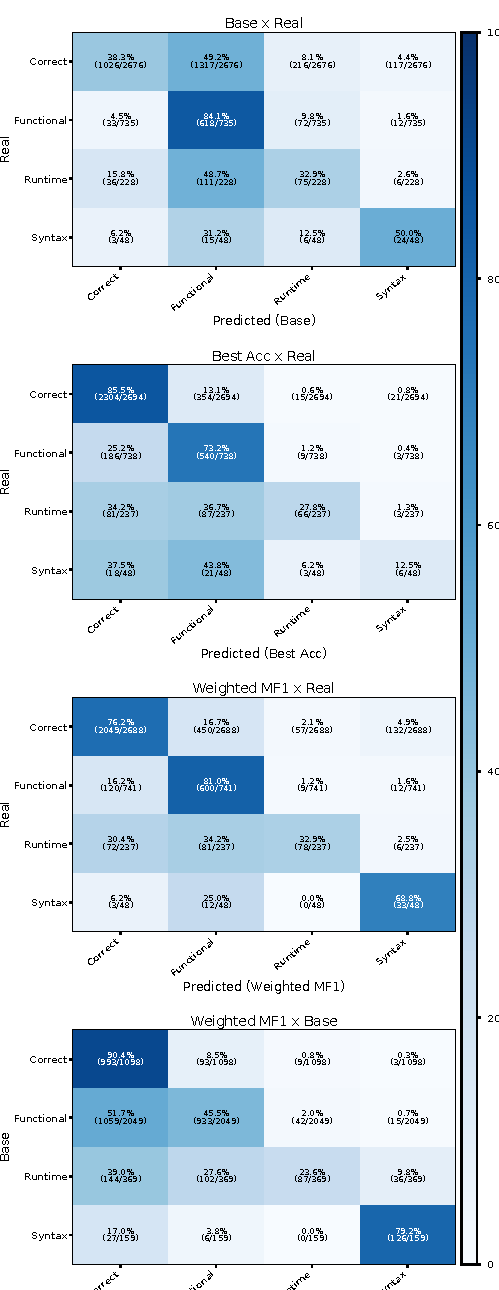
\includegraphics[width=\columnwidth]{figures/confusion_matrices.pdf}
\caption{Row-normalized confusion matrices under a primary-label reduction (priority syntax, runtime, functional, correct). Each cell reports the proportion and the counts as predicted / reference total. The first three matrices use the ground truth as reference, and the last compares the Weighted MF1 predictions against the base predictions. The number of evaluated samples differs slightly across matrices (Base 3{,}687; Best Acc 3{,}717; Weighted MF1 3{,}714; Weighted MF1 vs Base 3{,}675) because unparsable model outputs were excluded from the primary-label reduction.}
\label{fig:confusion}
\end{figure}

The dataset used for training is strongly imbalanced. Correct samples represent 72.4\% of the records, followed by Functional Error with 21.3\%, Runtime Error with 6.6\%, and Syntax Error with only 1.5\%. Because Accuracy favors predictions of the dominant class, a model trained on this distribution can learn to play safe and predict Correct most of the time. This motivated the evaluation of different training strategies. The split is performed at the task level, so all samples of a given programming task belong to a single split, and balancing is applied only to the training split, while validation and test remain intact.

The first search optimized validation Accuracy using the standard causal loss and the original class distribution. The search explored the base model, LoRA rank, alpha, dropout, learning rate, epochs, and bias configuration. The best configuration used Gemma 4 E4B with $r=16$, $\alpha=16$, dropout 0.1, learning rate $1\times10^{-4}$, 3 epochs, and bias \texttt{none}, reaching a validation Accuracy of 66.6\%. Figure~\ref{fig:confusion} shows that the Accuracy-oriented model shifts its decision boundary toward the dominant Correct class. In the base model, only 38.3\% of the Correct samples remain Correct, while 49.2\% are confused with Functional. Best Acc reduces Correct to Functional from 49.2\% to 13.1\% and also reduces Correct to Runtime (8.1\% to 0.6\%) and Correct to Syntax (4.4\% to 0.8\%), which explains where the Accuracy gain comes from. The cost is visible in the reverse direction: Functional to Correct rises from 4.5\% to 25.2\%, Runtime to Correct from 15.8\% to 34.2\%, and Syntax to Correct from 6.2\% to 37.5\%. The model did not simply learn Correct better; it began to favor Correct as an output.

Because per-class performance remained unbalanced, a second search optimized Macro-F1 instead. This search kept the same data distribution without explicit balancing and used the \texttt{label\_weighted} strategy with a class weight of 3.0. The best configuration used Gemma 4 E4B with $r=8$, $\alpha=8$, dropout 0.1, learning rate $1\times10^{-4}$, 3 epochs, and bias \texttt{none}, reaching a validation Macro-F1 of 52.4\% and a validation Macro Recall of 54.9\%.

The comparison between the two optimization objectives, presented in Table~\ref{tab:rq2_detection} and in Figure~\ref{fig:confusion}, clarifies how strongly the training objective changes the detector profile. Best Acc maximizes global performance, with 77.8\% Accuracy, 50.9\% Macro-F1, and 85.5\% Correct Recall. Weighted MF1 reduces Correct Recall to 76.2\% but increases Functional Recall from 73.2\% to 81.0\%, Runtime Recall from 27.8\% to 32.9\%, and Syntax Recall from 12.5\% to 68.8\%. The confusion matrices show that Weighted MF1 also reduces the tendency of Best Acc to absorb minority classes into Correct: Functional to Correct falls from 25.2\% to 16.2\%, and Syntax to Correct falls from 37.5\% to 6.2\%. In contrast to Best Acc, the Macro-F1-oriented model partially reverses the tendency to collapse minority classes into Correct. The optimization objective therefore changes not only the aggregate score but the classes the detector learns to recognize, and this is one of the main findings of this RQ.

Runtime remains the least stable class across training strategies. In the base model, Runtime is predicted as Functional in 48.7\% of cases and as Runtime in 32.9\%. Best Acc shifts Runtime toward Correct (34.2\%) and keeps only 27.8\% as Runtime, while Weighted MF1 keeps 32.9\% as Runtime and sends 30.4\% to Correct and 34.2\% to Functional. Fine-tuning changes where Runtime samples are misclassified, but does not produce an improvement comparable to that observed for Correct or Syntax. Syntax, in turn, is highly sensitive to the training strategy: it ranges from 11.8\% recall under Accuracy-oriented training to 64.7\% under Macro-F1-oriented training.

A third strategy changed the training distribution itself, reducing the number of Correct examples, removing Syntax, and testing proportions such as 1:1:1 and 1:3:3, with the goal of increasing the relative representation of the minority classes. The Balanced Acc model reached 67.8\% Accuracy, 38.1\% Macro-F1, 74.4\% Correct Recall, 65.8\% Functional Recall, 15.2\% Runtime Recall, and 0\% Syntax Recall. The Balanced MF1 model reached 63.7\% Accuracy, 36.0\% Macro-F1, 68.6\% Correct Recall, 65.8\% Functional Recall, 13.9\% Runtime Recall, and 0\% Syntax Recall.

Explicit balancing did not outperform the previous strategies. Both Accuracy and Macro-F1 decreased, Runtime detection also degraded, and Syntax reached 0\% because the class was removed from training. This suggests that simply rebalancing examples does not guarantee better learning, and that removing Correct examples may discard important information about the dominant class. In this setting, changing the objective and the loss was more effective than changing the dataset distribution. Objective-oriented training was more effective than explicit dataset balancing.

Syntax deserves separate discussion. The class is extremely rare, and many cases classified as Syntax result from an incompatible output format or structure rather than syntactically invalid Python. This makes the class small, heterogeneous, and difficult to learn, and highly sensitive to the training objective. The results illustrate this sensitivity: Best Acc reached 11.8\% Syntax Recall, Weighted MF1 reached 64.7\%, and the balanced models reached 0\%. These cases are not reclassified; the observed behavior only reflects how the training strategy interacts with a rare and heterogeneous class.

The overall effect of fine-tuning can be summarized by comparing the base and specialized models. The Gemma 4 E4B base model obtained 45.9\% Accuracy and 37.0\% Macro-F1. The Best Acc model reached 77.8\% Accuracy and 50.9\% Macro-F1, while Weighted MF1 reached 73.5\% Accuracy and 54.2\% Macro-F1. Fine-tuning therefore produces a substantial gain, and the specialization strongly changes the ability to recognize Correct, with Weighted MF1 producing the most balanced detector and Best Acc producing the strongest Accuracy. The deltas relative to the base model confirm this effect: Best Acc gains 31.9 percentage points of Accuracy, 13.9 of Macro-F1, and 47.3 of Correct Recall, while losing 17.3 of Functional Recall and 35.3 of Syntax Recall. Weighted MF1 gains 27.6 of Accuracy, 17.2 of Macro-F1, 37.9 of Correct Recall, and 17.6 of Syntax Recall. The balanced models gain around 21.9 and 17.8 of Accuracy but lose more than 20 points of Functional Recall and 47 of Syntax Recall.

The last matrix in Figure~\ref{fig:confusion} compares the Weighted MF1 predictions directly against the base predictions and should be interpreted as a prediction transition, not as correctness. It shows that among the samples the base model labeled as Correct, 90.4\% remain Correct; among those labeled as Functional, 51.7\% are reclassified as Correct by Weighted MF1; among those labeled as Runtime, only 23.6\% remain Runtime; and among those labeled as Syntax, 79.2\% remain Syntax. The largest behavioral shift therefore occurs among samples originally labeled as Functional by the base model, which are frequently reclassified as Correct. This does not imply an error by itself; it only shows how the decision behavior changed. Fine-tuning does not simply improve the detector: it changes its decision behavior, and different optimization objectives produce distinct error profiles.

\textbf{Answer to RQ3.} Specialized training substantially improves SLM-based error detection, but the resulting detector is highly sensitive to the optimization objective and to the class-imbalance strategy. Accuracy-oriented fine-tuning favors the dominant Correct class, whereas Macro-F1-oriented training yields more balanced performance across error categories. Explicit dataset balancing did not outperform objective-based weighting in the evaluated setting.

\subsection{RQ4: How do large language models compare with SLMs in error detection?}
\label{sec:rq4}

All models were evaluated on the same dataset, with the same prompt, the same protocol, and the same metrics, which allows a direct comparison between the two groups. The large models are DeepSeek V4.1 Flash, with 552B backbone parameters, and MiMo V2.5, with 310B parameters. Their results, presented in Table~\ref{tab:rq2_detection}, are compared with the best SLMs. DeepSeek V4.1 Flash obtained 75.5\% Accuracy, 51.0\% Macro-F1, and 47.7\% Macro Recall, while MiMo V2.5 obtained 51.5\% Accuracy, 39.7\% Macro-F1, and 61.1\% Macro Recall. Among the SLMs, Muse Glimmer 30B reached 73.1\% Accuracy and 53.8\% Macro-F1, Best Acc reached 77.8\% Accuracy, and Weighted MF1 reached 73.5\% Accuracy and 54.2\% Macro-F1. Larger models therefore did not show consistent superiority over the SLMs. DeepSeek is competitive in Accuracy, but it does not surpass Best Acc and it remains below Muse Glimmer and Weighted MF1 in Macro-F1, while MiMo is well below the best SLMs in Accuracy.

The large models also exhibit very different profiles across classes. DeepSeek V4.1 Flash reached 89.3\% Correct Recall, 51.6\% Functional Recall, 14.8\% Runtime Recall, and 35.3\% Syntax Recall, showing a strong tendency to recognize Correct. MiMo V2.5 reached 47.2\% Correct Recall, 79.7\% Functional Recall, 21.5\% Runtime Recall, and 96.1\% Syntax Recall, being particularly strong in Functional and Syntax. Neither model solves the Runtime problem, as both remain close to the low rates observed for the SLMs. As in RQ2, the detection behavior remains strongly class-dependent. The difficulty in detecting runtime errors persists even when moving from SLMs to substantially larger models.

The comparison between specialization and scale is the most informative. Weighted MF1 reached 73.5\% Accuracy, 54.2\% Macro-F1, and 62.9\% Macro Recall, while DeepSeek reached 75.5\% Accuracy, 51.0\% Macro-F1, and 47.7\% Macro Recall, and MiMo reached 51.5\% Accuracy, 39.7\% Macro-F1, and 61.1\% Macro Recall. Increasing the number of parameters by orders of magnitude does not guarantee higher detection capability. The specialized SLM Weighted MF1 surpasses both large models in Macro-F1, and Best Acc surpasses both in Accuracy. This suggests that specialization for the task can be more important than simply increasing scale. These conclusions should be stated with caution, since only two large models were evaluated. In the evaluated setting, specialization appears to compensate for model scale.

\textbf{Answer to RQ4.} Larger LLMs did not consistently outperform SLMs in error detection. Their performance remained strongly class-dependent, particularly for runtime errors. In the evaluated setting, specialized SLMs matched or surpassed substantially larger models in aggregate metrics, suggesting that task specialization can partially compensate for model scale.


\input{sections/5_conclusion}

\bibliographystyle{apalike}
\bibliography{refs}

\end{document}
